% ----------------------------------------------------------
% Modelagem
% ----------------------------------------------------------
\chapter{Modelagem e Implementação}
\label{chap:model}
% ----------------------------------------------------------

Como mencionado no \textbf{Capítulo \ref{chap:abordagem}}, a proposta do presente trabalho consiste na implementação de um algoritmo de \textit{deep reinforcement learning} para treinar um agente que seja capaz de aprender a jogar um jogo em \textit{Allegro.} A inspiração para o mesmo vem do trabalho realizado pelo \textit{Deep Mind} e publicado no artigo \cite{play-atari-drl-deepmind}, onde foi implementado uma IA capaz de jogar diferentes jogos Atari 2600. Assim, será implementado um sistema semelhante voltado para jogos em \textit{Allegro}.

O atual capítulo consiste em uma contextualização do ambiente e sistema a ser implementado, seguido de uma elaboração da modelagem matemática da abordagem proposta no \textbf{Capítulo \ref{chap:abordagem}} e, por fim, uma discussão sobre como o sistema foi implementado.

\section{\textit{Contextualização}} % (fold)
\label{sec:contextualizacao}


\subsection{O Jogo} % (fold)
\label{sub:o_jogo}

O ambiente escolhido para treinamento do modelo foi o jogo \textit{Frogger}. A escolha do mesmo foi feita tendo em vista sua simplicidade, tendo em vista as limitações de implementação (\textbf{Seção \ref{sub:limitacoes}}). A \textbf{Figura \ref{fig:frogg}} mostra a posição inicial do jogo utilizado. O agente controla o quadrado verde iniciado no centro inferior da tela, e tem como objetivo alcançar o topo da tela sem colidir com nenhum obstáculo, os quais são iniciados com tamanho e posições aleatórias.

\begin{figure}[h]
  \centering
  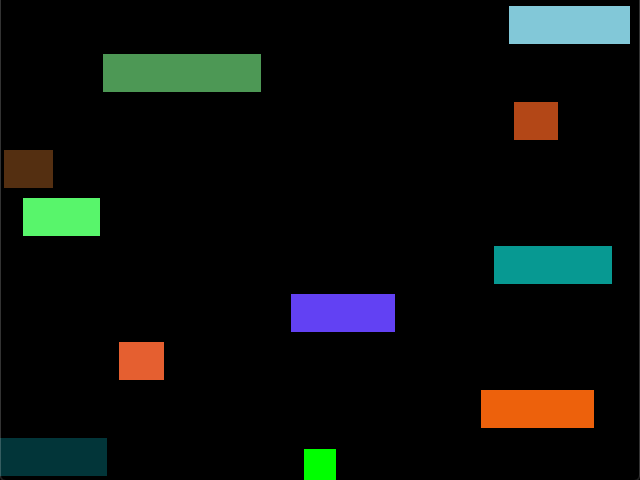
\includegraphics[width=.6 \textwidth]{conteudo/imgs/frogg_ini_state.png}
  \caption[Jogo \textit{Frogger}]{Exemplo do jogo \textit{Frogger} utilizado. O jogador controla o quadrado verde no centro inferior da tela, enquanto os outros retângulos coloridos são os obstáculos}
  \label{fig:frogg}
\end{figure} 

 As condições de parada, ou seja, os estados que constituem os estados finais do jogo são:

 \begin{itemize}
   \item Estados onde ocorra uma colisão do agente com o ambiente;
   \item Estado onde o agente atravessou o topo da tela (uma posição acima da última linha observável do jogo).
 \end{itemize}

 Por fim, as recompensas para ações durante o jogo foram definidas inicialmente da seguinte forma:

 \begin{itemize}
 	\item $r=-0.05$ caso o agente realize uma ação que o mantenha na mesma linha que se encontrava previamente. Essa recompensa negativa foi estipulada com o objetivo a desmotivar o agente a permanecer longos períodos de tempo sem progredir;
 	\item $r=1$ caso o agente realize uma ação que o aproxime verticalmente de seu objetivo;
  \item $r=-1$ caso o agente realize uma ação que o distancie verticalmente de seu objetivo;
 	\item $r=-1$ caso o agente realize uma ação que o leve a colidir com algum obstáculo (independente da direção que se movimentou);
 	\item $r=10$ caso o agente alcance seu objetivo.
 \end{itemize}

 % subsection o_jogo (end)
 
 \subsection{\textit{Allegro Learning Enviroment}} % (fold)
\label{sub:allegro_learning_enviroment}

Conforme descrito no \textbf{Capítulo \ref{chap:abordagem}}, será utilizada um \textit{Allegro Learning Enviroment} (ALE) que funcionará como intermédio entre o jogo e a IA. Essa ferramente tem como base a ferramente implementada por \cite{silva:amb-jd-allegro}, que foi modificada para atender as necessidades especificas do sistema atual. O ALE terá as seguintes funções principais:

\begin{itemize}
  \item Fornecer os valores de $\mathcal{A} = \{1,\cdots ,K\}$, que representa o conjunto de ações possíveis para o agente; 
  \item Determinar a posição da tela do jogo e realizar a captura das imagens que servirão como observações de estado para o agente;
  \item Executar um novo jogo para cada episódio de treinamento;
  \item Executar as ações estabelecidas pelo agente;
  \item Processar os dados do jogo incluindo: observação de cada instante de tempo, calcular a recompensa do atual estado do jogo, informação sobre quando um episódio é finalizado.
\end{itemize}

% subsection allegro_learning_enviroment (end)

% section reinforcement_learning (end)

\section{Modelagem Matemática} % (fold)
\label{sec:modelagem_matematica}

% \subsection{Aprendizagem por Reforço}

Como elaborado anteriormente, no aprendizado por reforço é desenvolvido um agente que irá interagir com um ambiente $\varepsilon$, nesse caso o jogo em \textit{Allegro}, a partir de uma sequência de ações, observações e recompensas.
Em cada etapa de tempo, o agente seleciona uma ação do conjunto de ações legais do jogo, $\mathcal{A} = \{1,\cdots ,K\}$. A ação é executada, modificando o estado do ambiente e pontuação do jogo.
%Em geral, $\varepsilon$ pde ser estocástico.
O estado interno do jogo não é observado pelo agente, este observa apenas uma imagem $x_t \in \mathbb{R}^d$, que é um vetor de valores de pixel brutos que representam a tela do estado atual do jogo. Além disso, o agente recebe uma recompensa $r$ que representa a alteração na pontuação do jogo.  

Em outras palavras, um agente explora um jogo, e é treinado tentando maximizar as recompensas nesse jogo. Este ciclo é ilustrado na \textbf{Figura \ref{rl-diagram-2}}.

\begin{figure}[h]
  \centering
  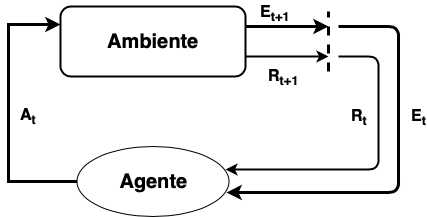
\includegraphics[width=.6 \textwidth]{conteudo/imgs/rl-diagram.png}
  \caption[Diagrama de aprendizagem por reforço]{Diagrama de aprendizagem por reforço elaborada melhor no \textbf{Capítulo \ref{chap:abordagem}}
  }
  \label{rl-diagram-2}
\end{figure}

% Em resumo, no \textit{loop} de \textit{feedback} mostrado na \textbf{Figura \ref{rl-diagram-2}}, os subscritos indicam as etapas de tempo $t$ e $t + 1$, cada uma das quais se refere a estados diferentes: o estado no momento $t$ e o estado no momento $t + 1$. 
% A ação $A_t$ de um agente é determinada por sua \textbf{política} $\pi$, que por sua vez é uma função que depende do estado atual do sistema $E_t$. A política de um agente tem como objetivo maximizar a \textbf{função de valor} $Q(s,a)$ que é calculada utilizando o \textbf{sinal de recompensa} $R_t$. O ambiente se comporta como um sistema caixa preta que transforma uma ação executada no estado atual $A_t$, no próximo estado $E_{t+1}$ e uma recompensa $R_{t+1}$

% \subsection{Processos de Decisão de Markov e a Equação de Bellman} % (fold)
% \label{sub:processos_de_decisão_de_markov}
% % subsection processo_de_decisão_de_markov (end)


É importante ressaltar que a pontuação do jogo pode depender de toda a sequência anterior de ações e observações. O \textit{feedback} sobre uma ação só pode ser recebido depois de decorridos múltiplos de intervalos de tempo. Uma vez que o agente apenas observa as imagens da tela atual, a análise do estado do jogo em que se encontra pode ser mal-representada, ou seja, é difícil para o agente compreender totalmente a situação em que se encontra apenas da tela atual $x_t$. 
Para solucionar esse problema, considera-se como um estado $s_t$ do jogo, uma sequência de ações e observações $s_t = (x_{t-n},a_{t-n},\cdots,a_{t-1},x_t)$, as quais serão utilizadas para treinar o agente, fornecendo-o um melhor contexto do estado em que se encontra. Esse formalismo dá origem a um processo de decisão de Markov (MDP), no qual cada sequência é um estado distinto. Como resultado, pode-se aplicar métodos de aprendizado por reforço padrão para MDPs, simplesmente usando a sequência completa $s_t$ como a representação do estado no tempo $t$.

Conforme descrito em \cite{play-atari-drl-deepmind}, o objetivo do agente é interagir com o jogo, selecionando ações de uma forma que maximize recompensas futuras. É feita a suposição padrão de que as recompensas futuras são descontadas por um fator de $\gamma$ por intervalo de tempo, e que o retorno descontado futuro é definido por: 
\begin{eqnarray}
	R_t=\sum_{t^{\prime}=t}^T \gamma^{t^{\prime}-t}\cdot r_{t^{\prime}}
\end{eqnarray}
onde T é o intervalo de tempo em que o jogo termina. 

A função de valor de ação ótima $Q^{*}(s, a)$ pode ser definida como o máximo retorno esperado alcançável de uma estratégia, depois de ver a sequência $s$ e se tomar alguma ação $a$:
\begin{eqnarray}
	Q^{*}(s, a)=max_\pi(\mathbb{E}[R_t | s_t=s,a_t=a,\pi])
\end{eqnarray}
onde $\pi$ é uma política que mapeia sequências para ações e $\mathbb{E}$ é a função de retorno esperado para um estado $s$ dado uma ação $a$.

A função de valor de ação ótima obedece a identidade da equação de Bellman. Essa se baseia na seguinte intuição: se o valor ótimo $Q^{*}(s_{t+1}, a_{t+1})$ da sequência $s_{t+1}$ na próxima etapa de tempo for conhecido para todas as ações possíveis ações $a_{t+1}$, então a estratégia ótima para o estado $s_t$ consiste em selecionar a ação $a_{t}$ que maximize o valor esperado futuro:
\begin{eqnarray}
	Q^{*}(s_t, a_t)= r + \gamma \cdot max(Q^{*}(s_{t+1},a_{t+1})|\forall a_{t+1})
  \label{eq:q_fun}
\end{eqnarray}

A ideia básica por trás de muitos algoritmos de aprendizagem por reforço é estimar a função de valor de ação, usando a equação de Bellman como uma atualização iterativa. Assim, dado um fator de aprendizagem $\alpha$, o valor de $Q(s,a)$, é atualizado durante o treinamento da seguinte forma:
\begin{eqnarray}
  Q_{i+1}(s_t,a_t) = Q(s_t,a_t) + \alpha[r + \gamma\cdot max_{a_{t+1}}Q(s_{t+1},a_{t+1}) - Q(s_t,a_t)]
  \label{eq:qlearning}
\end{eqnarray}

sendo que a subtração de $\gamma\cdot max_{a_{t+1}}Q(s_{t+1},a_{t+1})$ por $Q(s_t,a_t)$ é realizada para normalizar a atualização. 

Essa atualização dos valores da função de valor $Q$, permite que o algoritmo convirja para a função de ação ótima $Q_i \rightarrow Q^*$, com $i\rightarrow\infty$ \cite{sutton-barto-rl-intro}. Na prática, essa abordagem é totalmente impraticável, pois a função valoração é estimada separadamente para cada sequência, sem nenhuma generalização. Em vez disso, é comum usar um aproximador de função para estimar a função de valor de ação, $Q(s,a;\theta_t) \approx Q^*(s,a)$. Este aproximador toma a forma de uma rede neural, conhecida como uma \textit{Q-network}, onde $\theta_t$ refere-se aos parâmetros da rede neural (ou seja, os pesos e bias da rede). Assim, se os pesos são atualizados após cada passo de tempo, então chegamos ao conhecido algoritmo de \textit{Q-learning} \cite{Watkins-Dayan-Qlearning}. O valor de $\theta_t$ por sua vez pode ser atualizado conforme a \textbf{Equação \ref{eq:theta}}:
\begin{eqnarray}
  \theta_t = \theta_t + \alpha(r + \gamma\cdot max_{a_{t+1}}Q(s_{t+1},a_{t+1}) - Q(s_t,a_t))\nabla_\theta Q(s_t,a_t)
  \label{eq:theta}
\end{eqnarray}

Por fim, considerando a iteração de treinamento do agente usando \textit{Q-learning}, a política de seleção de ação é baseada apenas no valor máximo de $Q$ em qualquer estado dado. É concebível que, dada a inicial natureza estocástica do ambiente, o agente inicialmente tome decisões “ruins”. No entanto, como o agente nunca explorou ações melhores, ele pode interpretar que as decisões ruins tomadas inicialmente são boas e, daquele momento em diante, tomar somente aquelas decisões. Da mesma forma, mesmo que o agente tome ações iniciais ``boas'' ele pode acabar desenvolvendo uma política que prenda o agente em ótimos locais, ou seja, a ação determinada pela política é boa a curto prazo, mas a longo prazo ela é inferior ou até ruim. Esta política de seleção de ação é chamada de política gulosa.

Para evitar esses problemas, o agente deve explorar o maior número possível de estados e ações. Infelizmente, para problemas com um número muito grande de estados, explorar todos os estados e ações possíveis se torna impraticável. A política \textit{epsilon-greedy} na aprendizagem por reforço é basicamente a mesma que a política gulosa, exceto que há um valor épsilon que define uma probabilidade $1-\epsilon$ de uma ação ser escolhida aleatoriamente ao invés de definida pelo atual modelo. Dessa forma, o algoritmo força o agente a explorar diversos estados e ações, mesmo que estes não sejam a princípio recomendados pela função de valor $Q$. Dado um número suficientemente grande de ações, o agente terá explorado uma quantidade de estados suficiente para determinar uma política satisfatória. Essa abordagem permite também que o valor de $\epsilon$ seja atualizado e reduzido com o tempo de forma a permitir que o algoritmo se concentre mais em explorar as melhores soluções que encontrou. 

% section modelagem_matemática (end)

\section{Implementação} % (fold)
\label{sec:implementacao}

A modelagem descrita na \textbf{Seção \ref{sec:modelagem_matematica}}, fornece uma modelagem da rede neural proposta. O sistema nada mais é do que uma \textit{Deep Q Network} (DQN), que é constituída por uma \textit{Deep Neural Network} \cite{Goodfellow-et-al-2016} que utiliza a técnica de \textit{Q-learning}, onde cada nó de saída da rede corresponde à uma possível ação do agente. No entanto, um simples algoritmo usando o método descrito não converge para uma solução satisfatória. Nessa seção serão vistas algumas modificações para o algoritmo que o fará obter melhores resultados.

\subsection{\textit{Experience Replay}} % (fold)
\label{ssub:experience_replay}

Foi aplicada a técnica conhecida como \textit{Experience Replay} \cite{Lin1992ReinforcementLF}, onde as experiências do agente em cada passo de tempo, são armazenadas em um \textit{replay buffer}, que nada mais é do que uma lista de tuplas, cada tupla contendo o estado atual, a ação tomada, a recompensa obtida, e o próximo estado alcançado $(s_t,a_t,r_t,s_{t+1})$. Para treinar a DQN, recupera-se aleatoriamente um pequeno lote do \textit{replay buffer}, o qual é usado como dado de treinamento. A \textbf{Figura \ref{fig:exp_rep}} mostra o processo descrito.


\begin{figure}[h]
  \centering
  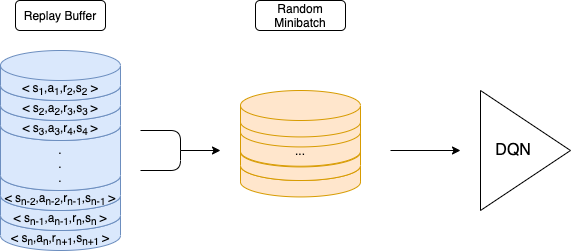
\includegraphics[width=.7 \textwidth]{conteudo/imgs/experience_replay.png}
  \caption[\textit{Experience Replay}]{Exemplo do processo de seleção de dados de treinamento. O histórico de estados, ações e recompensas obtido é salvo em um \textit{replay buffer}. Para treinar o agente, o algoritmo seleciona aleatoriamente um conjunto de amostras (\textit{minibatch}) de tamanho pré-definido que servirão como dados de treinamento da rede}
  \label{fig:exp_rep}
\end{figure} 

O \textit{buffer} implementado dessa forma é uma fila FIFO (\textit{First in, first out}), ou seja, quando ele atingir seu tamanho máximo, as novas entradas irão substituir as entradas mais antigas de forma a sempre manter o conjunto de dados mais atualizado. Além disso, antes de se inicializar o treinamento, o \textit{buffer} é inicializado com um tamanho mínimo, inicializado com amostras obtidas por um agente com política de ação aleatória.

O objetivo da alocação dos dados dessa forma é de fornecer à rede uma melhor distribuição de informação para o aprendizado. Um algoritmo de aprendizado simples recebe os dados de treinamento na mesma ordem em que são observados. Isso pode introduzir ao agente padrões ou correlações indesejadas, que podem afetar o processo de aprendizado do algoritmo. Assim, ao passar as observações de forma aleatória, a eficiência do algoritmo é melhorada. 


% subsubsection experience_replay (end)


\subsection{Pré-processamento de Imagens} % (fold)
\label{sub:preprocessamento}

Para treinar uma rede neural apartir de capturas de tela em cada instante do jogo, os dados de cada observação são extraídos dos pixels brutos exibidos. Um problema de utilizar imagens estáticas como observações é que isso limita a quantidade de informação que pode ser obtida do estado do jogo: não é possível determinar a velocidade ou direção na qual um objeto está se movendo. Para contornar essa situação, pode-se redefinir um estado como sendo um conjunto de $n$ instantes de tempo, como mencionado na \textbf{Seção \ref{sec:modelagem_matematica}}. 

Dado que a tela do jogo representa uma janela de $640\times480$ pixels, pode-se converter isso para um vetor de pixels RGB com dimensões $640\times480\times3$. Uma vez definido o estado como um conjunto de $n=4$ instantes, temos um vetor de entrada para rede neural de $640\times480\times3\times4=3686400$. Considerando que cada iteração do algoritmo deverá analisar um vetor desse tamanho, o custo computacional do treinamento do modelo é extremamente alto. Felizmente o vetor de entrada pode ser reduzido consideravelmente removendo algumas informações desnecessárias. Primeiramente, do ponto de vista do agente, a variação de cores do jogo é irrelevante. Sendo assim, pode-se converter a imagem para cinza, reduzindo o tamanho da matriz da imagem original de $640\times480\times3$ para $640\times480$. Por fim, podemos reduzir o tamanho dessa imagem, tendo em vista que informações redundantes de uma tela grande não são necessárias para treinamento do modelo. A \textbf{Figura \ref{fig:pross_imgs}} mostra o tratamento de uma imagem antes de ela ser adicionada ao estado que servirá de entrada para a rede.

\begin{figure}[h]
  \centering
  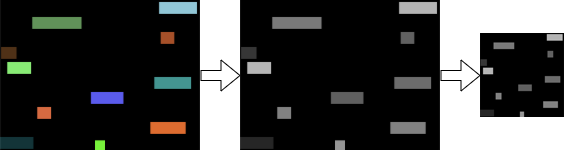
\includegraphics[width=.9 \textwidth]{conteudo/imgs/reducao_imgs.png}
  \caption[Processamento de Imagens]{Processamento das capturas de tela realizado antes das mesmas serem passadas como entradas para o treinamento da rede. Primeira imagem na esquerda é um exemplo da captura original, seguindo da mesma imagem transformada para cinza e por fim a imagem reduzida que será convertida para um vetor de pixels a ser passado como entrada para o modelo}
  \label{fig:pross_imgs}
\end{figure} 

Com isso, considerando uma redução para uma imagem final de $84\times84$ pixels, obtém-se um estado formado por um vetor de tamanho $84\times84\times4=28224$. Apesar do vetor final ainda apresentar um tamanho considerável, foi alcançado uma redução de $99.23\%$ na entrada do modelo, aliviando consideravelmente o custo computacional do sistema.

% subsection préprocessamento (end)

\subsection{\textit{Dueling Q Network}} % (fold)
\label{sub:rede_neural_dupla}

O problema do aprendizado por DQN está ligado à definição da sua função de valor. Da \textbf{Equação \ref{eq:q_fun}} temos:
$$Q^{*}(s_t, a_t)= r + \gamma \cdot max(Q^{*}(s_{t+1},a_{t+1})|\forall a_{t+1})$$

O problema da equação acima surge com o valor máximo. Esta parte da equação deve estimar o valor das recompensas para ações futuras se a ação $a$ for tomada a partir do estado atual $s_t$. O problema é que em muitos ambientes, a existência de um ruído aleatório, ou seja, uma variância no valor da recompensa, é inevitável. Assim, à medida que um agente explora um ambiente, ele não está observando diretamente $r$ ou $r_{futuro}$, mas algo como $r + \epsilon$, onde $\epsilon$ é o ruído ou o a variância da recompensa. Em tal ambiente, depois de jogar o jogo repetidamente, esperaríamos que a rede aprendesse a fazer estimativas imparciais do valor esperado das recompensas $E[r]$. Com isso, basta à rede escolher as melhores ações para recompensas atuais e futuras, apesar da presença de ruído.

É aqui que a operação de máximo é um problema: ela produz estimativas tendenciosas das recompensas futuras, não as estimativas imparciais de que necessitamos para obter os melhores resultados.
Considere o ambiente exemplificado pela \textbf{Figura \ref{fig:dqn_bias}} \cite{ThomasAndrew:adv_ml}. O agente começa no estado A e em cada estado pode mover-se para a esquerda ou direita. Os estados C e E são estados terminais. O jogo termina quando esses pontos são alcançados. Os valores de $r$ são as recompensas que o agente recebe ao fazer a transição de um estado para outro.

\begin{figure}[h]
  \centering
  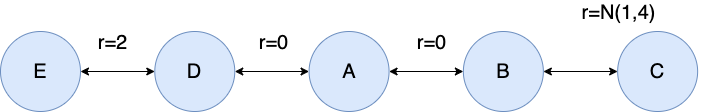
\includegraphics[width=.9 \textwidth]{conteudo/imgs/dqn_bias.png}
  \caption[\textit{Deep Q Network} bias]{Exemplo de um jogo que causa bias em uma DQN. O agente começa no estado A e em cada estado pode mover-se para a esquerda ou direita. Os estados C e E são estados terminais. O jogo termina quando esses pontos são alcançados. Os valores de $r$ são as recompensas que o agente recebe ao fazer a transição de um estado para outro. Figura extraída de \cite{ThomasAndrew:adv_ml}}
  \label{fig:dqn_bias}
\end{figure} 

Todas as recompensas são determinísticas, exceto as recompensas durante a transição dos estados B para C. As recompensas para essa transição é retirada aleatoriamente de uma distribuição normal com uma média de 1 e um desvio padrão de 4.

Sabemos as recompensas esperadas, $E[r]$ de qualquer ação de B para C é 1. No entanto, há uma variância associada à essas recompensas. Independentemente disso, em média, o agente deve aprender idealmente a sempre se mover para a esquerda de A, em direção a D e finalmente E, onde r sempre é igual a 2. No entanto, devido a função de máximo utilizada para calcular a função de valor, sempre é obtido o valor máximo dos sorteios aleatórios das recompensas e, com isso, o algoritmo tende a ser positivamente tendencioso e não dá uma indicação verdadeira dos valores esperados das recompensas para um movimento nesta direção (ou seja, 1). Como tal, um agente que usa a metodologia de \textit{Q-learning} não escolherá a ação ideal de A (ou seja, mover para a esquerda), mas tenderá a mover para a direita.

A solução para este problema foi proposta por \cite{vanhasselt2015deep}, e consiste na implementação de duas redes neurais, mas somente uma rede primária é treinada à cada iteração, enquanto a segunda rede, chamada de rede objetivo, é treinada com menos frequência. Esse processo ajuda a estabilizar os pesos da rede objetivo.

A arquitetura conhecida como \textit{Dueling Q}, é uma melhoria para a rede neural dupla. Utiliza-se a mesma metodologia de uma rede alvo e primária, com atualizações periódicas ou combinação dos pesos da rede alvo com os pesos da rede primária. No entanto, ele incorpora dois conceitos importantes na arquitetura da rede. Estas são as funções de vantagem e valor:

\begin{itemize}
  \item \textbf{Função de vantagem $A(s,a)$}: A função de vantagem é o benefício relativo de escolher uma determinada ação no estado $s$ sobre as outras ações possíveis no mesmo estado.
  \item \textbf{Função de valor V(s)}: A função de valor é o valor de estar no estado s, independente dos benefícios relativos das ações nesse estado
\end{itemize}

A função $Q(s,a)$ se torna então, uma adição dessas duas funções:

\begin{eqnarray}
  Q(s,a) = V(s) + A(s,a)
\end{eqnarray}

A motivação de dividir essas duas funções explicitamente na arquitetura é que pode haver estados inerentemente bons ou ruins para o agente estar, independentemente do benefício relativo de quaisquer ações nesse estado. Por exemplo, em um determinado estado, todas as ações podem fazer com que o agente "morra" em um jogo - este é um estado inerentemente ruim de se estar, e não há necessidade de desperdiçar recursos computacionais tentando determinar a melhor ação neste estado . O inverso também pode ser verdadeiro. Idealmente, esta “divisão” em função de vantagem e função de valor deve ser aprendida implicitamente durante o treinamento. No entanto, a arquitetura \textit{Dueling Q} torna essa divisão explícita, o que atua para melhorar o treinamento.

\subsection{Arquitetura Final} % (fold)
\label{ssub:arquiterura_final}

De acordo com as especificações descritas acima, a arquitetura final do modelo pode ser observada na \textbf{Figura \ref{fig:diagrama_rede}}. Pode-se observar que na arquitetura implementada, foram utilizadas camadas comuns de redes neurais convolucionais que realizam o processamento de imagens. A saída dessas camadas é então achatada e rede então se bifurca em um fluxo de função de valor $V(s)$ e um fluxo de função de vantagem $A(s,a)$. A saída desses fluxos separados é então agregada em uma camada especial, antes de finalmente produzir os valores Q da rede.

\begin{figure}[h]
  \centering
  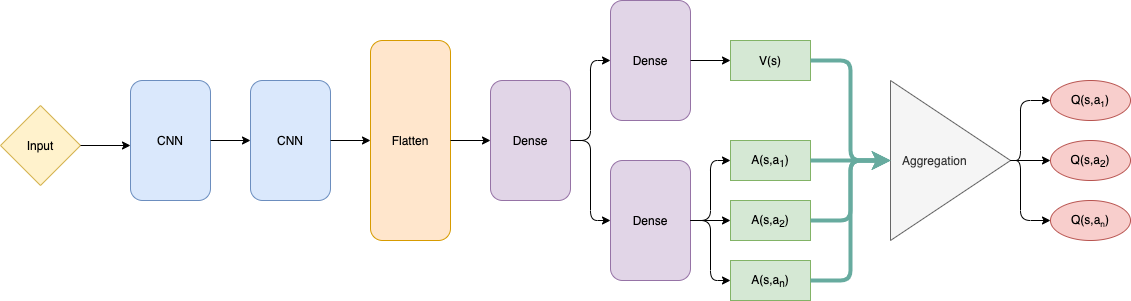
\includegraphics[width=1 \textwidth]{conteudo/imgs/diagrama_rede.png}
  \caption[Diagrama da arquitetura final da rede implementada]{Diagrama da arquitetura final da rede implementada}
  \label{fig:diagrama_rede}
\end{figure} 

A partir da arquitetura descrita acima, os \textbf{Algoritmos \ref{alg:main}} e \textbf{\ref{alg:train}} mostram o pseudocódigo do sistema implementado. O \textbf{Algoritmo \ref{alg:main}} mostra o corpo da função principal, enquanto o \textbf{Algoritmo \ref{alg:train}} descreve a função de treinamento do modelo.

\begin{algorithm}[H]
    \SetAlgoLined
    Inicializa o ambiente\\
    Inicializa a rede primária\\
    Inicializa a rede objetivo\\

    \For{episodio = 1:NUM\_EPISODIOS }{
      \While{jogo não termina}{
        ação $\leftarrow$ modelo.obtemAcao(estado,$\epsilon$)\\
        proximaObservacao, recompensa, fim $\leftarrow$ ambiente.executaAcao(ação)\\
        proximoEstado $\leftarrow$ obtemEstado(estado,proximaObservacao)\\[.3cm]

        experienceReplay.adicionaTupla(estado,ação,recompensa,proximoEstado,fim)\\[.3cm]

        treinaModelo()
      }
    }
   \caption{Corpo Principal}
   \label{alg:main}
  \end{algorithm}

  \begin{algorithm}[H]
    \SetAlgoLined
    $<s_t,a_t,r_t,s_{t+1},fim>$batch  $\leftarrow$ experienceReplay.obtemBatch()\\
    \eIf{fim}{
      $y \leftarrow r_t$
    }
    {
      $y \leftarrow r_t + \gamma\cdot max_{a_{t+1}}Q(s_{t+1},a_{t+1})$
    }

    \# Gradiente descendente\\
    $\Delta\theta\leftarrow\frac{\partial}{\partial\theta}(y - Q(s,a))^2$\\[.3cm]

    Atualiza os pesos da rede
   \caption{treinaModelo}
   \label{alg:train}
  \end{algorithm}

% subsubsection arquiterura_final (end)


% subsection rede_neural_dupla (end)


\subsection{Limitações} % (fold)
\label{sub:limitacoes}

A implementação do sistema apresentado enfrentou uma série de limitações que fogem do alcance do desenvolvedor. Os desafios encontrados durante a implementação, assim como as soluções para circunver estes problemas, quando possível, são descritas abaixo.

\subsubsection{Tempo de Treinamento e Limitações de Hardware} % (fold)
\label{subsub:tempo_de_treinamento_e_limitações_de_hardware}

O principal obstáculo enfrentado foi o tempo de treinamento do sistema. Devido a complexidade e número de entradas do problema, o modelo pode levar dias ou semanas para alcançar uma política ótima. Como mencionado anteriormente, cada estado é formado por quatro imagens constituindo os quatro últimos instante do jogo. Mesmo após a conversão para cinza e compressão das imagens de $640\times480$ para $84\times84$ pixels, isso ainda deixa cada estado com um vetor de entrada de tamanho $84\times84\times4=28224$. Tudo isso considerando um tamanho de tela bem modesto e um jogo sem informações muito complexas (quando comparado com um jogo 3D por exemplo).

Esses problemas são agravados ainda mais devido às limitações do hardware onde o sistema foi implementado. A máquina utilizada possui as seguintes especificações:

\begin{itemize}
  \item MacBook Air 2015;
  \item Processador: 1.6 GHz Dual-Core Intel Core i5;
  \item Memória: 4 GB 1600 MHz DDR3;
  \item Sistema Operacional: macOS Catalina | Windows 10.
\end{itemize}

Como pode ser observado, trata-se de uma máquina com poder computacional limitado, com relativamente pouca memória, um processador bastante simples e sem uma placa de vídeo dedicada. Todas essas limitações acabam levando à um tempo de treinamento ainda maior.

% subsection tempo_de_treinamento_e_limitações_de_hardware (end)

\subsubsection{Integração do Sistema com o Jogo em \textit{Allegro}} % (fold)
\label{subsub:integração_do_sistema_com_o_jogo}

Como mencionado no \textbf{Capítulo \ref{chap:abordagem}} e em \ref{sub:allegro_learning_enviroment}, a comunicação entre a IA, implementada em \textit{Python}, e o jogo, implementado em C, é realizada através de um \textit{Allegro Learning Enviroment} (ALE). No entanto, como o ALE também é implementado em \textit{Python}, a integração dos dois sistemas apresenta algumas limitações.

Primeiramente, o cálculo da recompensa seria, idealmente, calculado pelo programa do jogo e passado para o ALE. No entanto, qualquer saída do programa em C só é recebida pelo ALE uma vez que o programa é finalizado ao fim de um episódio. Isso inviabiliza o calculo em tempo real de qualquer estado que não sejam os estados iniciais ou finais. Por esse motivo o calculo das recompensas de cada estado deve ser feito pela ALE, o qual é realizado através um simples registro da posição do agente no jogo.

Outro problema que surge da integração da ALE com o o jogo é o processamento das imagens e que, por sua vez, acaba exacerbando ainda mais o problema de tempo de treinamento descrito em \ref{subsub:tempo_de_treinamento_e_limitações_de_hardware}. Ao iniciar um novo episódio, o programa em C leva alguns instantes para ser lançado e ter seu estado inicial renderizado. Portanto, para garantir que a observação do estado inicial do jogo seja realizada propriamente, a ALE aguarda $0.1s$ para garantir que o programa foi inicializado propriamente e $0.2s$ após o jogo ser concluído. Esse tempo torna-se considerável a medida que o número de episódios de treinamento aumentam. Um treinamento com dez mil episódios, por exemplo, recebem um aumento de cerca de $50$ minutos. 

Além disso, os jogos em \textit{Allegro} devem ter seus dados processados manualmente. A \textbf{Figura \ref{fig:process_img}} mostra um diagrama que indica todos os passos do processamento de dados necessários para gerar as informações de cada estado do jogo.

\begin{figure}[h]
  \centering
  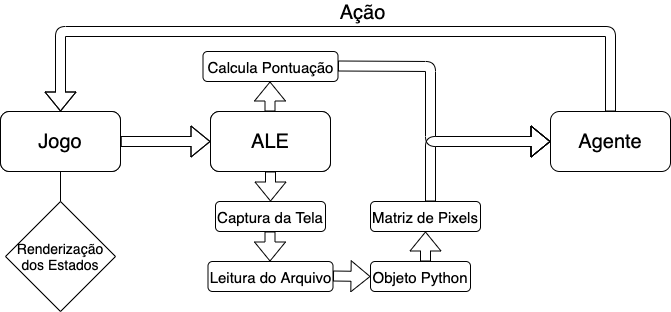
\includegraphics[width=.8 \textwidth]{conteudo/imgs/processamento_imgs.png}
  \caption[Diagrama de processamento de imagens]{Diagrama mostrando como as informações de cada estado são processadas antes de serem passadas para a IA. Isso inclui executar o programa em C, transmitir os comandos de ação do agente para o jogo, renderizar as imagens em cada instante do jogo, realizar a captura de tela, acessar os arquivos onde essas imagens foram salvas, transformar os dados desse arquivo para um objeto em \textit{Python}, transformar o objeto em uma matriz com os dados da imagem para somente então os mesmos serem passados para o modelo a ser treinado}
  \label{fig:process_img}
\end{figure} 

Jogos em Atari 2600 que possuem um emulador em \textit{Python} que são capazes de gerar um vetor de observação que contém os dados de cada instante do jogo sem a necessidade de renderizar as imagens do mesmo \cite{brockman2016openai}. O mesmo não pode ser dito para os jogos em \textit{Allegro}. Para obter as observações dos estados do jogo, deve-se executar o programa em C, renderizar cada estado do jogo e realizar a captura de tela dos mesmos, e realizar o processamento dessas imagens antes desses dados serem passados para a IA. Todo o processo deve ser realizado para cada instante que deseja-se observar e calcular uma ação. Para evitar que o alto tempo de processamento dos dados leve a alguma perda de informações que prejudique o treinamento (como o agente permanecer inativo por um longo período de tempo enquanto calcula o próximo movimento), o jogo foi alterado de forma que cada quadro (\textit{frame}) do jogo seja atualizado somente quando o agente realizar uma ação. Esse formato de implementação acaba constituindo um \textit{trade-off}: a perda de informações do agente é minimizada, mas o tempo de execução de cada episódio aumenta.

% subsection integração_do_sistema_com_o_jogo_em_tex (end)

% subsection limitações (end)
% section implementação (end)
